\chapter{Theoretische Grundlagen}
In diesem Kapitel werden die theoretischen Grundlagen der Zeitreihe und möglicher Analyseformen, genauso wie die Theorie der Referenzmodellierung und die Systematik der Anforderungserhebung und  Produktauswahl erläutert. \Todo{https://bi-survey.com/challenges-big-data-analytics}

\section{Grundlagen der Datenanalyse}\label{chap:GrundlagenDatenanalyse}

Mathematisch ausgedrückt besteht eine Zeitreihe (im Englischen auch \enquote{time series} genannt) aus einer endlichen Menge an zeitlich aufsteigend sortierten Messwerten $x_{t_1},x_{t_2},...,x_{t_T};  x_{t_k} \in \mathbb{R}^n, k=1,2,...,T$, wofür $t_1 < t_2 < t_T $ gilt.\footcite[Vgl.][1]{Deistler.2018b} 
Zeitreihendaten sind in verschiedenen Feldern zu finden, beispielsweise im Bereich der Aktienmärkte, wo die Preise der einzelnen Kurse abgebildet werden, im Bereich der Gesundheitsforschung, wo die Ansteckungsrate ansteckender Krankheiten wie Covid-19 verfolgt wird oder im Bereich der Sozialwissenschaften, in welchen der Verlauf von Geburtsraten über die Zeit analysiert werden soll.\footcite[Vgl.][1]{Shumway.2017b} 
In \autoref{abb:BeispielZeitreihe} findet sich beispielhaft die Zeitreihe der zwei messbaren Feinstaubkategorien von null bis ein Uhr am 01.01.2020 in Stuttgart.

\begin{figure}[H]
\centering
\includegraphics[width=\textwidth]{graphics/Feinstaub-Stuttgart.png}
\caption{Beispielhafte Feinstaubwerte in der Stunde nach Silvester 2020 in Stuttgart-Mitte}
\label{abb:BeispielZeitreihe}
\end{figure}

Die möglichen Anwendungen in der Informatik sind ebenfalls vielzählig. So können über virtuelle oder physikalische Sensoren Messwerte, wie beispielsweise die CPU Auslastung eines gegebenen Servers über die Zeit oder Temperaturmessungen eines \ac{IoT} Gerätes über die Zeit gemacht und gespeichert werden. So nehmen mit zunehmender Digitalisierung von Fertigungslinien in Fabriken auch die Messwerte von Sensoren zu, die dort übermittelt und ausgewertet werden müssen.

Ein wichtiges Merkmal von Zeitreihen ist die Distanz zwischen den Messwerten, im Sinne der Messfrequenz, in welcher Daten betrachtet werden. \TodoW{belegen} Ist eine Zeitreihe äquidistant, wurde mit gleichbleibender Frequenz gemessen und die zeitliche Distanz zwischen einzelnen Messwerten ist gleich. Für die in dieser Arbeit diskutierten Auswertungsarten wird eine Äquidistanz der gemessenen Daten angenommen, da andernfalls ein Bias/eine Verfälschung bei der Analyse nicht ausgeschlossen werden kann. Gleichfalls ist es technisch möglich, einzelne, nicht äquidistante Messwerte auszusortieren oder fehlende Messwerte zu interpolieren. Die in \autoref{abb:BeispielZeitreihe} abgebildete Zeitreihe ist äquidistant, da die Werte alle 124 Sekunden erhoben wurden.

Es ist von zwei vorliegenden Typen von Zeitreihendaten auszugehen. Zum einen existiert der mit Zeitstempel versehene Messwert, welcher einen oder in manchen Fällen auch mehrere diskrete Messwerte mit Zeitstempel der Erfassung übermittelt. 
Zum anderen existieren auch Ereignisse, welche keine Messwerte enthalten, sondern Ergebnisse einer Vorauswertung innerhalb des übermittelnden Systems sind. 
So wäre ein Ereignis beispielsweise ein niedriger Batteriestand eines verbundenen Sensors. 
Abhängig von der Vorauswertung werden Ereignisse einmal, nach Auftreten mit Zeitstempel oder periodisch mit Zeitstempel bis zum Beheben der Ursache versendet.\footnote{Siehe auch \anhangref{anhang:interview-peter-24.03.2021}}

\subsection{Analysewert verarbeiteter Daten}\label{chap:datenwert}

Bei der Verarbeitung von Daten ist zu beachten, dass der Wert, bzw. die Erkentnisse die aus den Daten abgleitet werden können, über die Zeit reduziert wird. \footcite[Vgl. auch im Folgenden][]{NucleusResarchInc..2012} Gemäß \citeauthor{NucleusResarchInc..2012} haben dabei verschiedene Unternehmen verschiedene Zeiträume, in denen Daten nützlich sind, da sie sich in eine von drei Entscheidungstempi einkategorisieren lassen.\footcite[Vgl. auch im Folgenden][3]{NucleusResarchInc..2012} Die Entscheidungstempi sind taktisch, operativ und strategisch. Beim taktischen Entscheidungstempo werden Änderungen sehr schnell, nahe Echtzeit getroffen und implementiert. Im Gegensatz dazu werden Entscheidungen der operativen und strategischen Entscheidungstempi respektive erst in Tagen bzw. Wochen oder innerhalb einem Quartal oder länger implementiert. Je nach Entscheidungstempo sind Analysen von eingehenden Daten also wesentlich früher notwendig oder können beispielsweise auch nur einmal täglich erstellt werden.

Für Unternehmen mit taktischem Entscheidendungstempo haben, gemäß der in \autoref{abb:DataHalflife} gezeigten Befragungsergebnisse von \citeauthor{NucleusResarchInc..2012}, Daten nach maximal 30 Minuten die Hälfte des Wertes eingebüßt.\footcite[Vgl. auch im Folgenden][6]{NucleusResarchInc..2012} Für operative Entscheidungstempi ist die durchschnittliche Halbwertszeit nach acht Stunden erreicht, für strategische Entscheidungstempi nach ca. 56 Stunden, also nach über 2 Tagen.



\begin{figure}[H]
\centering
\includegraphics[width=\textwidth]{graphics/half-life-data.pdf}
\caption[Die Halbwertszeit von Daten]{Die Halbwertszeit von Daten\footnotemark}
\label{abb:DataHalflife}
\end{figure}
\footnotetext{Mit Änderungen entnommen aus: \cite{NucleusResarchInc..2012}}
Aus diesen abweichenden Halbwertszeiten und damit aus den abweichenden Zeiträumen, in denen die erhobenen Daten den höchsten Wert haben, ergibt sich die Notwendigkeit von verschiedenen Datenverarbeitungsstrategien, um entsprechend taktischen, operativen oder strategischen  Entscheidenden die werthaltigsten Daten als Entscheidungsgrundlage zu präsentieren.

\subsection{Arten der Auswertung}\label{chap:auswertungsarten}
Diese Arbeit soll anhand einiger weniger Auswertungen demonstrieren, wozu die jeweilige Referenzarchitektur und die verwendeten Dienste fähig sind. Im Folgenden werden dazu einige einfachere Auswertungsmethoden für Zeitreihendaten vorgestellt. Die Zeitreihenanalyse und einsetzbare Werkzeuge werden im statistischen Sinn von weiterführenden Werken, wie von \citeauthor{Shumway.2017} behandelt. Es ist davon auszugehen, dass auch weiterführende Auswertungen wie fourieranalytischen Methoden, sofern in der jeweiligen Umgebung bereits vorhanden oder programmierbar, eingesetzt werden können.


\subsubsection{Median und Quantile}
Eine der wichtigsten statistischen Lageparameter sind die Quantile eines Datensatzes und der Median, welcher ein spezielles, 50 prozentiges Quantil ist. 
Innerhalb eines gewissen Betrachtungsfensters können für Zeitreihendaten, wie für viele andere Datensätze auch, Quantile und der Median erfasst werden. 
Das Quantil erfasst mit der jeweiligen Prozentangabe und dem zugehörigen, ermittelten Wert die Grenze an Werten, die kleiner sind. 
Bei einem 75-\%-Quantil von $2$ wären entsprechend nur 25\% der sich im Datensatz befindlichen Daten größer als $2$. 
Da ein Median das 50-\%-Quantil ist, bildet der Median entsprechend die Grenze ab, bei welcher 50\% der Werte im Datensatz kleiner und der Rest größer ist. In \autoref{abb:quantile} sind das 25, 50 und 75-\%-Quantil einer Messreihe gezeigt.
\begin{figure}[H]
\centering
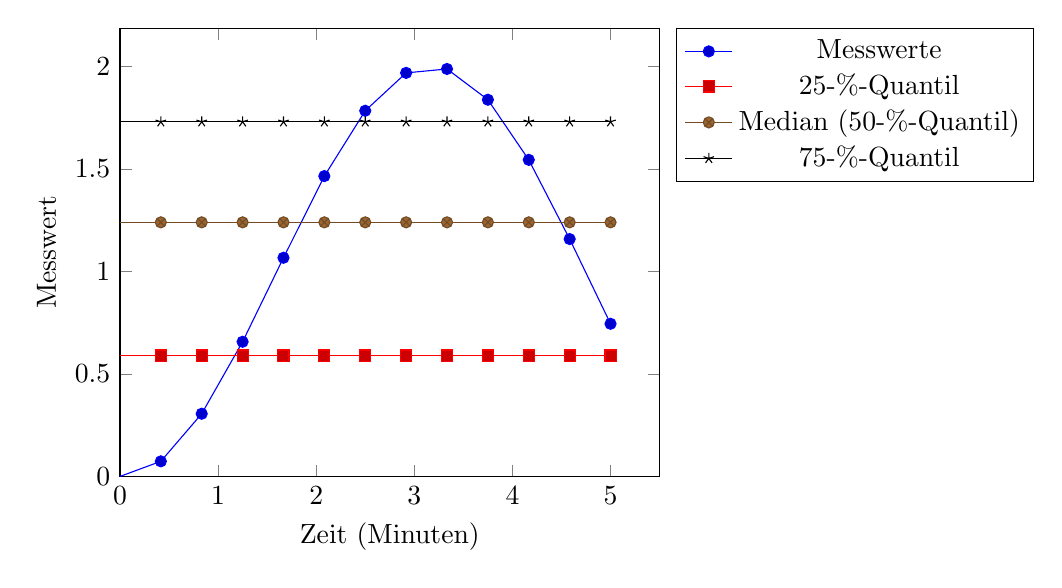
\begin{tikzpicture}
    \begin{axis}[
    xlabel=Zeit (Minuten),
    ylabel=Messwert,
    xmin=0, 
    ymin=0,
    legend pos=outer north east]
        \addplot {sin(deg(x-1.6))+1}; 
        \addplot {0.5899082};
        \addplot {1.2392493};
        \addplot {1.72939505};
        \legend{Messwerte,25-\%-Quantil,Median (50-\%-Quantil),75-\%-Quantil}
    \end{axis}
\end{tikzpicture}
\caption{Median und Quantile angewendet auf eine Messreihe}
\label{abb:quantile}
\end{figure}

Gängig in der Datenanalyse als Sonderform der Quantile sind die sogenannten Perzentile, welche in einprozentigen Schritten existieren. Häufig verwendet werden insbesondere das 90-\% und das 99\% Perzentil.

\subsubsection{Anomaliedetektion}
Eine weitere gängige Datenanalysemethode ist die Anomaliedetektion. 
Dabei kann jeder Datenpunkt als Anomalie gesehen werden, der die Komplexität eines Modells, welches die Daten beschreibt, substantiell erhöhen würde.\footcite[Vgl.][]{Guha.2016} Verwandt ist dabei das Feld der \enquote{Ausreissererkennung}/outlier detection. 
Verwendet werden können dabei diverse Methodiken. Innerhalb von \ac{AWS} Diensten wird zur Anomalieerkennung ein Algorithmus basierend auf Random Cut Forest verwendet.\footcite[Vgl.][1]{Guha.2016} Weitere Methodiken wären aber auch Random Walk oder Logik basierend auf Standardannahmen.\footcite[Vgl.][]{Moonesinghe.2006}\nzitat\footcite[Vgl.][]{Angiulli.2008} Anomalien können kausal mit unterliegenden Problemen z.B. des Sensors zusammenhängen, weshalb es wichtig ist, auch abseits von den in \autoref{chap:schwellwert} gezeigten Schwellwertüberprüfungen die Daten auf Anomalien zu prüfen.

\begin{figure}[H]
\centering
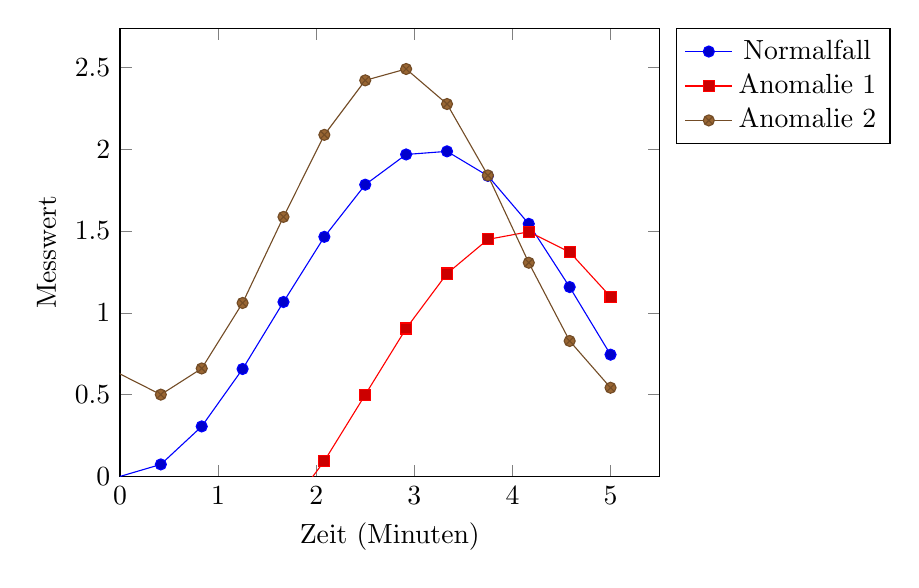
\begin{tikzpicture}
    \begin{axis}[
    xlabel=Zeit (Minuten),
    ylabel=Messwert,
    xmin=0, 
    ymin=0,
    legend pos=outer north east]
        \addplot {sin(deg(x-1.6))+1}; 
        \addplot {sin(deg(x-2.5))+0.5};
        \addplot {sin(1.3*deg(x-1.6))+1.5};
        \legend{Normalfall,Anomalie 1,Anomalie 2}
    \end{axis}
\end{tikzpicture}
\caption{Zu erkennende Anomalien einer Messreihe}
\label{abb:anomalie}
\end{figure}

Abgebildet in \autoref{abb:anomalie} sind zwei Anomalien, die direkt in mehreren Punkten vom Normalfall abweichen.
\subsubsection{Schwellwertüberschreitung}\label{chap:schwellwert}
Bei vielen gemessenen und sonstig erfassten Zeitreihendaten, bei denen akzeptierbare Werte und Wertbereiche, die Aktionen erfordern bekannt sind, sind Schwellwerte bereits ausreichend oder komplementär verwendbar. Dabei wird, wie in \autoref{abb:Schwellwerte} gezeigt, ein Schwellwert definiert (in diesem Fall $1.75$). Zusätzlich dargestellt ist eine Karenzzeit von 12 Sekunden. Erst nach kontinuierlicher Überschreitung des Schwellwerts von 12 Sekunden wird ein Alarm ausgelöst. 
\begin{figure}[H]
\centering
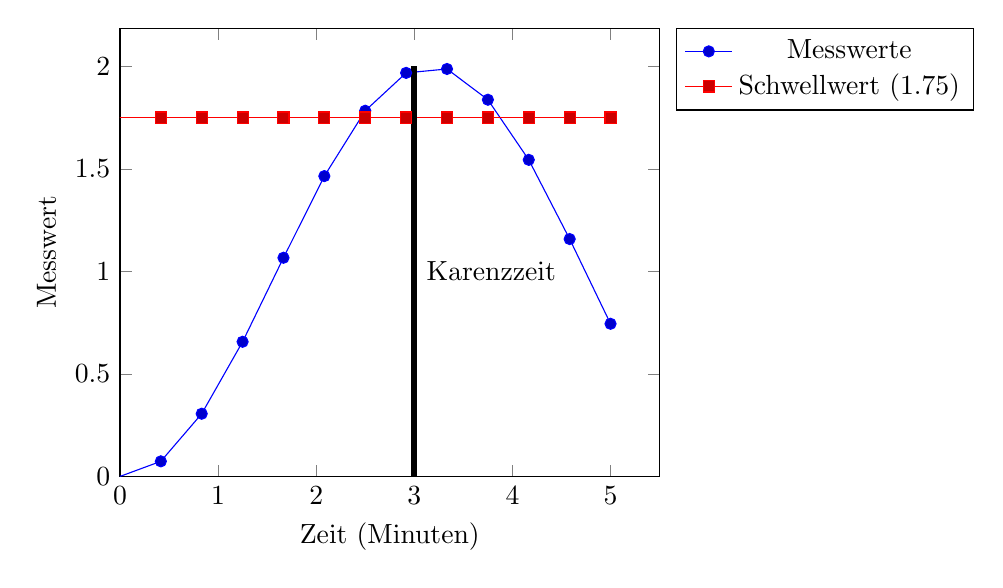
\begin{tikzpicture}
    \begin{axis}[
    xlabel=Zeit (Minuten),
    ylabel=Messwert,
    xmin=0, 
    ymin=0,
    legend pos=outer north east]
        \addplot {sin(deg(x-1.6))+1}; 
        \addplot {1.75};
        \draw [line width=0.8mm, black](axis cs:3,0) -- node[right]{Karenzzeit} (axis cs:3,2);
        \legend{Messwerte,Schwellwert ($1.75$)}
    \end{axis}
\end{tikzpicture}
\caption{Schwellwertüberschreitung mit Karenzzeit einer Messreihe}
\label{abb:Schwellwerte}
\end{figure}
Gleichzeitig ist es aber auch möglich, zählerbasiert einen Alarm/eine Aktion auszulösen. Bei einer Messdistanz von angenommenen 10 Sekunden und dreifacher Auslösung wäre eine 30 sekündige Karenzzeit ebenfalls implementierbar.

\subsubsection{Trenderkennung/gleitender Durchschnitt}
Gleitende Durchschnitte, wie in \autoref{abb:gleitendeDurchschnitte} gezeigt, sind eine Form der Kurvenglättung. Sie glätten ausreissende Kurven und ermöglichen einen groben Trend der vorliegenden Daten anhand der Steigung der geglätteten Kurve vorauszusagen.
\begin{figure}[H]
\centering
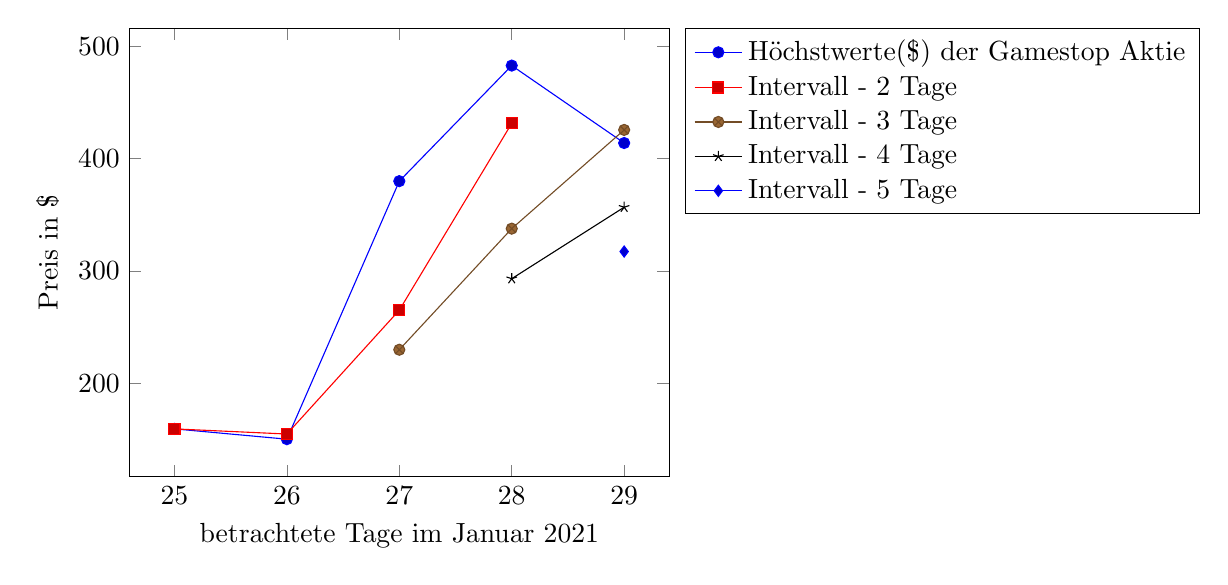
\begin{tikzpicture}
    \begin{axis}[
    xlabel=betrachtete Tage im Januar 2021,
    ylabel=Preis in \$,
    legend pos={outer north east},
    legend cell align={left}
]
        \addplot coordinates {
        	(25, 159.18)
        	(26, 150)
        	(27, 380)
        	(28, 483)
        	(29, 413.98)
        };
        
        \addplot coordinates {
        (25, 159.18)
        (26, 154.59)
        (27, 265)
        (28, 431.5)
        };
        \addplot coordinates {
        (27,229.7266667)
        (28,337.6666667)
        (29,425.66)
        };
        
        \addplot coordinates {
        (28,	293.045)
        (29,	356.745)
        };
        
        \addplot coordinates {
        (29,	317.232)
        };
        \legend{Höchstwerte(\$) der Gamestop Aktie,Intervall - 2 Tage,Intervall - 3 Tage,Intervall - 4 Tage,Intervall - 5 Tage};
    \end{axis}
\end{tikzpicture}
\caption{Gleitender Durchschnitt des Tageshöchstwertes eines Aktienkurses}
\label{abb:gleitendeDurchschnitte}
\end{figure}






\subsection{Bestehende Referenzarchitekturkategorien}\label{chap:bestehende_ras}
Im Bereich der Streamingarchitekturen gibt es bereits etablierte Referenzarchitekturen, welche verschiedene mögliche Aufbauarten einer Verarbeitung von Streaming/Zeitreihendaten zeigen.

\begin{figure}[H]
\centering
\includegraphics[width=\textwidth]{graphics/Lambda-Reference-Architecture.pdf}
\caption[Die $\lambda$-Datenstreaming Referenzarchitetktur]{Die $\lambda$-Datenstreaming Referenzarchitetktur.\footnotemark}
\label{abb:LambdaStreaming}
\end{figure}
\footnotetext{Mit Änderungen entnommen aus: \cite[][28]{Marz.2015}}

Die von \citeauthor{Marz.2015} vorgestellte $\lambda$/Lambda-Architektur, welche in \autoref{abb:LambdaStreaming} gezeigt wird, ist dabei eine der sehr bekannten Referenzarchitekturen. 
Der Name ist dabei nicht mit dem \ac{AWS} Dienst Lambda zu verwechseln, sondern ist wohl auf den gedrehten Buchstaben $\lambda$ zurückzuführen, also \reflectbox{\rotatebox[origin=c]{270}{$\lambda$}}.\footcite[Vgl. auch im Folgenden][]{Berle.27.11.2017} Die $\lambda$-Architektur sieht, ausgehend von den hereingeladenen Daten, zwei verschiedene Wege für die Daten vor. 
Zum einen den \enquote{Speed Layer}, welcher Daten direkt nach dem Eingang verarbeitet und nicht im Layer selbst speichert, sondern nur Aggregate oder Ergebnisse zur Verfügung stellt. Zum anderen gibt es den \enquote{Batch layer}, in welchem Daten zuerst in einem Master dataset gespeichert werden und dann in einem festen Intervall (\enquote{Batch jobs}) ausgewertet werden. 
Verschiedene Datenverarbeitungsintervalle machen speziell im Sinne der verschiedenen, in \autoref{abb:DataHalflife} gezeigten, Datenhalbwertszeiten Sinn. So sind manche Auswertungen, die präzise historische Daten benötigen, in einem Batch layer besser möglich als in einem Speed layer. Der Speed layer bietet dagegen durch die Geschwindigkeit der Auswertungen die Möglichkeit, agil auf erkannte Ereignisse oder Veränderungen im Generellen zu reagieren.


\begin{figure}[H]
\centering
\includegraphics[width=\textwidth]{graphics/Kappa-Reference-Architecture.pdf}
\caption[Die $\kappa$-Datenstreaming Referenzarchitetktur]{Die $\kappa$-Datenstreaming Referenzarchitektur.\footnotemark}
\label{abb:KappaStreaming}
\end{figure}
\footnotetext{Mit Änderungen entnommen aus: \cite{Kreps.2014}, \cite{Berle.27.11.2017}}

Die $\kappa$/Kappa Referenzarchitektur von \citeauthor{Kreps.2014}, dargestellt in \autoref{abb:KappaStreaming} basiert auf der $\lambda$-Architektur, spart jedoch den \enquote{Batch layer} mit zugehörigen \enquote{Batch jobs} aus. 
Das Konzept von einem Master Dataset existiert dabei weiterhin, jedoch in Form von Nachrichten, die in einem Messagebroker gespeichert werden. Analysen werden in Form von einzeln versionierten Jobs über die vorhandenen Werte erstellt. 
Wird die Analyse in irgendeiner Weise verändert (z.B. durch Codeanpassungen) werden alle zwischengespeicherten Nachrichten erneut durch eine neue, unveränderliche Version des Jobs analysiert. Diese Unveränderlichkeit hat den Vorteil, dass keine unerwünschten Seiteneffekte durch Analysen, die gegenseitig Ergebnisse überschreiben, auftreten. 



\begin{figure}[H]
\centering
\includegraphics[width=\textwidth]{graphics/OLAP-Reference-Architecture.pdf}
\caption[OLAP Referenzarchitetktur]{OLAP Referenzarchitetktur.\footnotemark}
\label{abb:OLAPStreaming}
\end{figure}
\footnotetext{Mit Änderungen entnommen aus: \cite{Kreps.2014}}

Aus der $\lambda$ Referenzarchitektur lässt sich auch eine, zur $\kappa$ Architektur gegenteilige Architektur aufzeigen. Diese ist im Stile des von \citeauthor{Codd.1993} geprägten \ac{OLAP} gehalten. Diese Architektur basiert, wie in \autoref{abb:OLAPStreaming} gezeigt, auf einer periodischen Verarbeitung der Daten im Master dataset. Dieses Vorgehen ist bei traditioneller Datenanalyse weit verbreitet, bietet jedoch womöglich wichtige Einsichten erst, nachdem die Datenhalbwertszeit bereits überschritten wurde.


\subsection{Echtzeitverarbeitung}
Gemäß der in \autoref{abb:KappaStreaming} gezeigten $\kappa$-Architektur gibt es Nutzungsfälle, in welchen eine reine Echtzeitauswertung basierend auf einer Datenquelle, wie beispielsweise einem Messagebroker, Sinn machen kann. \citeauthor{Belur.2020} sieht dabei vier verschiedene Verwendungszwecke, in welchen die niedrige Verarbeitungslatenz besonders wichtig ist und den maximalen Wert aus den Daten zieht.\footcite[Vgl. auch im Folgenden][]{Belur.2020} Durch Echtzeitreporting und die Erstellung von Dashboards können aktuelle Daten schnell übersichtlich aufbereitet werden. Mittels erstellter Regeln, die Schwellwertüberschreitungen und Anomalien detektieren, können Nutzende benachrichtigt werden, sobald es zu einer Abweichung kommt. Ebenfalls sinnvoll ist der Einsatz von Machine Learning zum Auffinden von Mustern in Daten, was verbesserte Anomalierkennung, Vorhersagen und ähnliche Features ermöglicht. Ein weiterer valider Usecase der $\kappa$-Architektur ist die Transformation von Daten in gewisse Zielformate, um beispielsweise Drittsysteme anzusprechen.


\subsection{Batch Verarbeitung}

Gemäß der in \autoref{abb:OLAPStreaming} gezeigten \ac{OLAP} Architektur, gibt es, wie für die Echtzeitverarbeitung auch nutzende Unternehmen, die ein Entscheidungstempo mit weiterem Horizont haben. Für diese Entscheidungstypen ist dabei wichtig, dass eine Analyse möglichst viele historische Daten umfasst. Es ist dabei aber zweitrangig, wie zeitnah diese erstellt werden kann. 
Eine gängige Möglichkeit um effizient alte Daten zu analysieren, stellen \ac{OLAP} Datenbanken dar, welche durch spezielle Indexstrukturen und Optimierungen auf komplexe lesende Abfragen bei großen Datenmengen optimiert wurden. \footcite[Vgl.][5\psq]{Codd.1993} Mittels dieser \ac{OLAP} Datenbanken lassen sich dank der jeweiligen Abfragesprachen und -dialekte komplizierte Abfragen realisieren. Bekanntes Beispiel für so eine Abfragesprache wäre \ac{SQL}, welche einige verschiedene Implementierungen (Dialekte) hat, die verwendet werden können. 

\section{Referenzarchitektur}\label{theorie:referenzmodellierung}
Nach \citeauthor{Bass.2010} ist eine Referenzarchitektur ein spezialisiertes Referenzmodell, wie in \autoref{abb:RelationshipsReferenceModel} welches in Softwarearchitekturen instanziiert werden kann. \footcite[Vgl.][S.~17~f.]{Bass.2010} 

\begin{figure}[H]
\centering
\includegraphics[width=0.66\textwidth]{graphics/Relationships-reference-models.pdf}
\caption[Beziehungen zwischen Referenzmodellen, Architekturpatterns, Referenzarchitekturen und Softwarearchitekturen]{Beziehungen zwischen Referenzmodellen, Architekturpatterns, Referenzarchitekturen und Softwarearchitekturen.\footnotemark}
\label{abb:RelationshipsReferenceModel}
\end{figure}
\footnotetext{Mit Änderungen entnommen aus: \cite[][18]{Bass.2010}}

In diesem Kapitel sollen deshalb die theoretische Definition des Referenzarchitekturbegriffs, genauso wie mögliche Vorgehensmodelle betrachtet werden.



\subsection{Referenzmodelle}

Gemäß des konstruktionsprozessorientierten Referenzmodellbegriffs von \citeauthor{vomBrocke.2003} ist ein Referenzmodell als solches zu erkennen, wenn der Gegenstand und/oder\footnote{Die Verwendung von \enquote{und/oder} wurde hier gewählt, da der Autor der Quelle das \enquote{oder} aus der boolschen Algebra gewählt hat um explizit beide Fälle einzuschliessen.} der Inhalt des Referenzmodells bei der Konstruktion des Gegenstandes und/oder des Inhaltes eines zu konstruierenden Anwendungsmodells wiederverwendet werden kann.\footcite[Vgl.][34]{vomBrocke.2003} Dabei hat ein Referenzmodell einen Empfehlungscharakter und stellt eine \enquote{best practice} dar.\footcite[Vgl.][31]{vomBrocke.2003} 

Ein Referenzmodell kann nach \citeauthor{vomBrocke.2003} nicht objektiv allgemeingültig sein und auch keinen objektiven Empfehlungscharakter haben, sondern muss subjektiv beurteilt werden.\footcite[Vgl. auch im Folgenden][31~f.]{vomBrocke.2003}  Dabei ist zumindest von den Interessensgruppen der Konstruierenden und der Nutzenden auszugehen, welche das Referenzmodell subjektiv unterschiedlich nach Allgemeingültigkeit und Empfehlungscharakter bewerten. Je nachdem welche Beurteilung höher gewichtet wird und früher einfließt, kann also entweder von der Situation ausgegangen werden, dass das Referenzmodell vom Konstruierenden zu einem solchen erklärt wird oder ein Modell, ob vom Konstruierenden beabsichtigt oder nicht, von den Nutzenden zu einem solchen erhoben wird.

\subsection{Grundsätze ordnungsgemäßer Referenzmodellierung}
\Todo{Grundsätze ordnungsgemäßer Modellierung/GoRM - siehe auch 148 vomBrocke.2003} \\
\textbf{=> Buch ist per Fernleihe bestellt, aber noch nicht da}


\subsection{Referenzarchitektur}
Der IEEE Standard 1471-2000 definiert Architektur im Kontext von softwareintensiven Systemen wie folgt:
\enquote{The fundamental organization of a system embodied in its components, their relationships
to each other, and to the environment, and the principles guiding its design and evolution.} \footcite[][3]{IEEEComputerSociety.2000}. Ein softwareintensives System wird dabei als jedes System, bei dem Software essentielle Einflüsse auf das Design, die Erstellung, das Deployment oder die Evolution des Systems hat.\footcite[Vgl.][1]{IEEEComputerSociety.2000}

Wird dieser Architekturbegriff auf bekannte Bereitstellungsmodi aus der Cloud, wie \ac{SaaS}, \ac{PaaS}, \ac{IaaS} oder \ac{FaaS} angewendet, wird klar, dass von einer Architektur im Sinne des IEEE Standards 1471-2000 ausgegangen werden kann, sobald Software involviert ist. Im Rahmen dieser Arbeit werden auch Dienste, die sich nach der NIST Cloud Definition unter \ac{SaaS} Dienste zählen lassen, behandelt. Als \ac{SaaS} Dienst gilt dabei jeder Dienst, bei dem Nutzende die unterliegende Infrastruktur nicht verwalten und die Applikation nur über limitierte Konfigurationen verwalten können. Sollte aber die Konfiguration mittels einer Programmiersprache bzw. Datenabfragesprache wie SQL erfolgen, ist die Bedingung erfüllt, dass Software wesentliche Einflüsse auf das System hat.


\citeauthor{Gallagher.2000} definiert eine Referenzarchitektur als eine generalisierte Architektur mehrerer Endsysteme, die eine oder mehrere Domänen teilen.\footcite[Vgl. auch im Folgenden][3]{Gallagher.2000} Die Referenzarchitektur definiert nach Sicht des Autors dabei die gemeinsame Infrastruktur der Endsysteme und die Schnitstellen der Komponenten, die in den Endsystemen enthalten sein sollen. Dabei ist eine Referenzarchitektur zu instanziieren, um eine spezifische Softwarearchitektur zu erstellen. Gallagher definiert die Aufgaben einer Referenzarchitektur wie folgt: Zum einen werden übergreifende Funktionen und Konfigurationen generalisiert und extrahiert und zum anderen wird eine kosteneffiziente und verlässliche Basis geschaffen, um Zielsysteme abzuleiten/zu instanziieren.\footcite[Vgl.][3]{Gallagher.2000}

\citeauthor{Trefke.2012} schränkt in seiner Definition die Instanziierung insoweit ein, dass individuelle Besonderheiten abstrahiert werden müssen, um eine Allgemeingültigkeit der Referenzarchitektur in einer speziellen Domäne zu erhalten.  \footcite[Vgl. auch im Folgenden][]{Trefke.2012} Zusätzlich fügt \citeauthor{Trefke.2012} der Referenzarchitektur als optionale Aufgaben die Definition von Leitlinien für die Verwendung, Evolution und Verantwortlichkeiten hinzu. Zurückgreifend auf \citeauthor{vomBrocke.2003} legt \citeauthor{Trefke.2012} fest, dass eine Referenzarchitektur als spezifischeres Referenzmodell seinen Empfehlungscharakter entweder durch Erfahrungen und hohe Nutzerakzeptanz oder durch Festsetzung durch Erschaffende erhält.

Nach \citeauthor{Angelov.2012} gibt es zwei Typen und damit verbundene Zielsetzungen der Referenzarchitektur: Die standardisierende Referenzarchitektur, welche darauf zielt eine Standardarchitektur für spezielle Anwendungsfälle zu schaffen und die unterstützende/erleichternde Referenzarchitektur, welche Personen in Architekturrollen unterstützen sollen, ähnliche Probleme leichter zu lösen.\footcite[Vgl. auch im Folgenden][S.~422~ff.]{Angelov.2012} Nach \citeauthor{Angelov.2012} sind standardisierende Referenzarchitekturen nicht zur Verwendung von innovativen, also kaum getesteten oder noch nicht von Experten akzeptierten Elementen geeignet. Die unterstützenden/erleichternden Referenzarchitekturen hingegen können solche innovativen Elemente durchaus verwenden und auch eine Technologievorauswahl treffen.

% Um einen möglichst hohen Nutzen stiften zu können, müssen die organisatorischen Rahmenbedingungen, in welchen ein Referenzmodell eingesetzt werden soll analysiert werden.\footcite[Vgl.][]{vomBrocke.2004}

%\Todo{What are inputs of a Reference Architecture? - Muller.2020}
\citeauthor{Muller.2020} empfiehlt eine Referenzarchitektur zur Generalisierung von vorhandenen Architekturen zu verwenden, schlägt aber für neue Technologien und Applikationen, die bislang in der Form kaum verwendet wurden ein inkrementelles Vorgehen vor.\footcite[Vgl. auch im Folgenden][7]{Muller.2020} Das inkrementelle Vorgehen von Muller beinhaltet dabei die Erstellung von Prototypen und inkrementelle Einholung von Feedback der Zielstakeholder.


\subsection{Qualitätskriterien von Referenzarchitekturen}\label{chap:qualitycriteria}
\citeauthor{Muller.2020} schlägt sieben Qualitätskriterien vor, welche von einer guten Referenzarchitektur erfüllt werden sollten:\footcite[Vgl. auch im Folgenden][8]{Muller.2020}
\begin{enumerate}
\item Verständlichkeit für eine breite, heterogene Gruppe an Stakeholdern (Kunden, Projektmanager, Entwickler, etc.)
\item Zugänglichkeit und Zugriff durch die Mehrheit der Organisation
\item Adressierung der Hauptprobleme der spezifischen Problemdomäne
\item Zufriedenstellende Qualität
\item akzeptabel
\item \enquote{up-to-date} und wartbar
\item wertschöpfend für den Betrieb
\end{enumerate}

\ac{AWS} definiert im Rahmen des sogenannten Well Architected Frameworks für verschiedene \enquote{Lenses}, also Spezialisierungen, Themenfelder, die bei exzellenten Architekturen zu beachten sind. Für Datenanalysen gibt es die Analytics Lens, welche entsprechend für Referenzarchitekturen genauso Anwendung finden sollte. Kriterien sind dabei die Folgenden:\footcite[Vgl.][6]{Ravirala.2020}:
\begin{itemize}
\item Automate data ingestion
\item Design ingestion for failures and duplicates => Siehe Robustness and fault tolerance
\item Preserve original source data
\item Describe data with metadata
\item Establish data lineage
\item Use the right ETL tool for the job
\item Orchestrate ETL workflows
\item Tier storage appropriately
\item Secure, protect, and manage your entire analytics pipeline
\item Design for scalable and reliable analytics pipelines => Scalability, robustness and fault tolerance
\end{itemize}


\subsection{Vorgehensmodell}

Nach \citeauthor{Muller.2020} hat eine Referenzarchitektur mehrere Dekompositionen, in beispielsweise eine funktionale, eine konstruktionsorientierte oder eine infrastrukturorientierte Komposition. Diese Dekompositionsschichten lassen sich ebenfalls in bekannten Architekturfframeworks wie arc42 finden, weshalb diese mit Anpassungen zur Visualisierung dienen sollen.

Zur Darstellung der verwendeten Produkte und Dienstleistungen von \ac{AWS} in den Referenzarchitekturen und dem Datenfluss soll die erste Stufe der Bausteinsicht des Architekturstandards arc42 verwendet werden. Das Konzept jener Bausteinsicht, also wie sie zu gestalten ist, findet sich in \autoref{abb:BausteinsichtStufe1}. In der finalen Umsetzung werden die offiziellen \ac{AWS} Icons die entsprechenden Services darstellen, die verwendet werden. Weitere Dekompositionsebenen, Beispiele und Kentnissammlungen die zu einer Referenzarchitektur gehören können unformalisierter beigefügt werden.

\begin{figure}[H]
\centering
\includegraphics[width=\textwidth]{graphics/Bausteinsicht.png}
\caption[Stufe 1 der Bausteinsicht in arc42]{Stufe 1 der Bausteinsicht in arc42.\footnotemark}
\label{abb:BausteinsichtStufe1}
\end{figure}
\footnotetext{Mit Änderungen entnommen aus: \cite{Starke.o.J.}}



Wie von \citeauthor{Muller.2020} vorgeschlagen und im vorherigen Unterkapitel erläutert, ist ein inkrementeller Ansatz unter Verwendung von Prototypen und kontinuierlichem Feedback der Zielstakeholder unerlässlich.\footcite[Vgl.][7]{Muller.2020} 

Sehr wichtig für eine Referenzarchitektur ist auch die Dokumentation, wie die Wiederverwendung zu handhaben ist. Ein möglicher Ansatz wäre dabei die gezielte Integration und Dokumentation von Variationspunkten, wie von \citeauthor{Webber.2001} vorgeschlagen.\footcite[Vgl.][24\psqq]{Webber.2001} Mittels der Variationspunkte kann eine statische Referenzarchitektur konstruiert werden, welche an spezifisch definierten Punkten angepasst werden muss, um einzigartige Architekturen zu erzeugen.\footcite[Vgl.][24]{Webber.2001} Dabei gibt es vier verschiedene Ansichten, aus denen Variationspunkte definiert werden können:\footcite[Vgl.][25\psq]{Webber.2001}
\begin{enumerate}
\item \label{view:first} Requirement-Variation-Point View
\item \label{view:second} Component-Variation-Point View
\item \label{view:third} Static-Variation-Point View
\item \label{view:fourth} Dynamic-Variation-Point View
\end{enumerate}
Dabei sind für diese Arbeit, in der keine implementierungsnahe (im Sinne von Programmierung) Softwarearchitektur entworfen wird, hauptsächlich die anforderungsbasierte und die komponentenbasierte Variationspunktsicht aus \autoref{view:first} und \autoref{view:second} wichtig. Die statische und dynamische Variationspunktsicht aus \autoref{view:third} und \autoref{view:fourth} agieren stärker auf Implementierungsebene, in dem beispielsweise mittels objektorientierter Programmierung Klassen bereitgestellt werden, von welchen geerbt werden kann und deren Verhaltensweisen durch z.B. Callbacks oder Parameterisierung des Aufrufes verändert werden kann.\footcite[Vgl.][25\psq]{Webber.2001} 

\renewcommand\#{\protect\scalebox{0.8}{\protect\raisebox{0.4ex}{\char"0023}}}

Variationspunkte können, wie in \autoref{abb:Variationspunkte} dargestellt innerhalb der verschiedenen, dargestellten Schichten wie folgt dargestellt werden:
\begin{figure}[H]
\centering
\includegraphics[height=1.33cm]{graphics/Variationpoints.pdf}
\caption{Darstellung Variationspunkte}
\label{abb:Variationspunkte}
\end{figure}
In den Architekturebenen werden entsprechend die Variationspunkte mit durchgängigen Nummern versehen, welche entsprechend vor dem \# stehen.





% Überleitung => generelle Referenzmodelle 
% => Empfehlungscharakter 
% => Anwendung Architektur 
% => Unterlegung Arc42 als Modellierungssprache



\section{Theorie der Anforderungserhebung}\label{chap:requirements}

Gemäß der in \autoref{chap:qualitycriteria} definierten Qualitätskriterien und der von \citeauthor{vomBrocke.2003} aufgestellten Allgemeingültigkeitskriterien kann ein Referenzmodell und damit auch eine Referenzarchitektur nicht objektiv allgemeingültig sein. Zusätzlich ergeben sich als weitere wichtige Eingaben zur Konstruktion eines Referenzmodells die Dekompositionstiefe und die Anwendbarkeit. Zusammen lassen sich diese Dimensionen als Kiviat Diagramm\footcite[Vgl.][33\psqq]{Kolence.1973}, wie in \autoref{abb:Dimensionen} gezeigt, abbilden. 

\begin{figure}[H]
\centering
\scalebox{0.75}{
    \spider{0}{0}{0}
}

\caption{Referenzarchitekturdimensionen}
\label{abb:Dimensionen}
\end{figure}

Ziel einer Referenzarchitektur sollte also sein, das optimale Verhältnis der drei Dimensionen für die Zielstakeholder zu finden und daraus eine Referenzarchitektur zu erstellen. Um dieses Ziel zu erreichen, sind Interviews mit Zielstakeholdern der SPIRIT/21 zu führen, welche dem Interviewleitfaden in \autoref{tab:intervieleitfaden} folgen. Im referenzierten Leitfaden stehen dabei Fragen mit einem F-Präfix für allgemeine Fragen und Fragen mit einem D-Präfix für Fragen in Bezug auf die drei Dimensionen. Kombiniert mit mindestens einem Review der Referenzmodelle werden die Modelle zu einem nutzenstiftenden Artefakt.



\begin{table}[H]
\centering
\begin{tabular}{|l|l|}
\hline
ID & Beschreibung \\ \hline
\multicolumn{2}{|c|}{\cellcolor[HTML]{ECF4FF}Allgemeine Fragen} \\ \hline
F1 & Rolle innerhalb der SPIRIT/21 \\ \hline
F2 & Anwendungsgebiete der Referenzarchitekturen \\ \hline
F3 & Kompatibilität der Referenzarchitekturen zueinander? \\ \hline
\multicolumn{2}{|c|}{\cellcolor[HTML]{ECF4FF}Priorisierungen} \\ \hline
P1 & Priorisierung der Qualitätskriterien (siehe \autoref{chap:qualitycriteria}) \\ \hline
P2 & Priorisierung der Datennutzungstypen (siehe \autoref{chap:GrundlagenDatenanalyse}) \\ \hline
\multicolumn{2}{|c|}{\cellcolor[HTML]{ECF4FF}Dimensionen der Referenzarchitekturen} \\ \hline
D1 & Anforderungen an Anwendung der Referenzarchitekturen \\ \hline
D2 & Anforderungen an Allgemeingültigkeit der Referenzarchitekturen \\ \hline
D3 & Dekompositionstiefe der Referenzarchitekturen \\ \hline
\end{tabular}
\caption{Interviewleitfaden für Schlüsselstakeholder}
\label{tab:intervieleitfaden}
\end{table}




\section{Vergleichsmethodik für die Produktauswahl}\label{chap:vergleichsmethodik}

\citeauthor{Marz.2015}, die bereits die $\lambda$-Architektur geprägt haben, haben folgende,erwünschte Eigenschaften eines Big Data Systems festegelegt:\footcite[Vgl.][7\psqq]{Marz.2015}
\begin{enumerate}
\item Robustness and fault tolerance

Systeme sollen Herausforderungen, wie beispielsweise Paralellität, Datenduplikate oder technische Ausfälle verkraften. Zusätzlich ist Resilienz gegenüber menschlichen Fehlern wünschenswert, so dass händische Änderungen rückgängig gemacht werden können (also beispielsweise Analysecode \enquote{immutable} ist).
\item Low latency reads and updates

Lesezugriffe auf Daten sollen mit niedriger Latenz stattfinden. Wie bereits beschrieben, kann aufgrund der Messdistanz eine Aktualisierung von Daten durchaus längere Zeit benötigen, jedoch sollte ein Big Data System in der Lage sein, Datenaktualisierungen mit niedriger Latenz durchzuführen.
\item Scalability

Das Big Data System sollte durch transparente oder intransparente Provisionierung weiterer Ressourcen in der Lage sein, gleiche Performance in verschiedenen Belastungssituationen zu liefern. Dies deckt sich mit einem der Kernversprechen der Public Clouds nach NIST Definition (\enquote{rapid elasticity}).\footcite[Vgl.][2]{Mell.2011}
\item Generalization

Ein Big Data System sollte in der Lage sein, verschiedene Anwendungen zu unterstützen. Da die Zielsetzung dieser Bachelorarbeit auf Zeitreihendaten aufbaut, welche wie in \autoref{chap:GrundlagenDatenanalyse} gezeigt, einen großen Einsatzspielraum haben, ist diese Bedingung bei ausreichender Generalisierung der Referenzarchitekturen erfüllt.
\item Extensibility

Das zu gestaltende Big Data System soll erweiterbar sein und neue Funktionen oder Änderungen ohne größeren Aufwand ermöglichen.
\item Ad hoc queries

Diverseste Abfragen sollen schnellstmöglich auf dem Datensatz der Big Data Anwendung möglich sein.
\item Minimal maintenance

Eine Big data Anwendung soll wartbar bleiben, indem Komplexität in den Kernkomponenten, welche nach Ansicht von \citeauthor{Marz.2015} zu erhöhtem Wartungsaufwand führt, möglichst gering ist.
\item Debuggability

Innerhalb eines Big Data Systems soll es möglich sein, nachzuverfolgen, wie Werte entstanden sind, um mögliche Fehler verfolgen zu können.
\end{enumerate}

% Kriterien von Lukas an ein Produkt:
% \begin{itemize}
% \item zufriedenstellende Integration mit AWS nativen Diensten (z.B. Monitoring)
% \item Möglichst serverless (wenig Maintenance Aufwand)
% \item skalierbarkeit auf 0 bis 10000
% \end{itemize}

% Anforderungen von Kunden
% \begin{itemize}
% \item Skalierbarkeit
% \item pay for what you use (no dead infra)
% \item transparente Fehler
% \end{itemize}

% \begin{itemize}
%     \item Übertragbarkeit (ggf. zwischen Clouds)
% \end{itemize}




=> Sortierte Tabelle mit Kriterien (geben Plus oder entsprechend Minuspunkte)
\begin{table}[H]
\centering
\begin{tabular}{|l|l|l|}
\hline
ID & Kriterium & Priorität \\ \hline
\#A & Robustness and fault tolerance & 11 \\ \hline
\#B & Scalability & 10 \\ \hline
\#C & möglichst serverless/pay for usage & 9 \\ \hline
\#D & Minimal maintenance & 8 \\ \hline
\#E & Debuggability/transparente Fehler & 7 \\ \hline
\#F & Extensibility & 6 \\ \hline
\#G & Low latency reads and updates & 5 \\ \hline
\#H & Ad hoc queries & 4 \\ \hline
\#I & Generalization & 3 \\ \hline
\#J & Integration mit AWS nativen Produkten & 2 \\ \hline
\#K & Übertragbarkeit zwischen Clouds (ISO 9126) (Anhang) & 1 \\ \hline
\end{tabular}
\caption{Prioritäten}
\label{tab:prioritaeten}
\end{table}

% \begin{table}[H]
% \centering
% \begin{tabular}{|l|l|l|}
% \hline
% \rowcolor[HTML]{ECF4FF} 
% Robustness and   fault tolerance & Scalability & möglichst serverless \\ \hline
% x/11 & x/10 & x/9 \\ \hline
% \rowcolor[HTML]{ECF4FF} 
% Minimal maintenance & Debuggability/transparente Fehler & Extensibility \\ \hline
% x/8 & x/7 & x/6 \\ \hline
% \rowcolor[HTML]{ECF4FF} 
% Low latency reads and updates & Ad hoc queries & Generalization \\ \hline
% x/5 & x/4 & x/3 \\ \hline
% \rowcolor[HTML]{ECF4FF} 
% Integration mit AWS & Übertragbarkeit (ISO 9126) & Summe \\ \hline
% x/2 & x/1 & \cellcolor[HTML]{DAE8FC}x \\ \hline
% \end{tabular}
% \caption{Bewertungsmatrix Produkt}
% \label{tab:bewertungsmatrix-produkt}
% \end{table}

\produktbewertung{Produkt}{x,x,x,x,x,x,x,x,x,x,x,x}

Ausgehend von den in \autoref{tab:prioritaeten} gezeigten Prioritäten, soll \autoref{tab:bewertungsmatrix-Produkt} verwendet werden um die jeweiligen Produkte zu bewerten.

\subsection{Featurevergleich}

\subsection{Performancevergleich}

\subsection{Kostenvergleich}

